% !TeX root = ../documento.tex
\chapter{Resultados e discuss\~ao}
\label{chap:resultados}

Este capítulo reúne os achados obtidos com a validação em simulação do controle digital de pressão hidráulica e com o desenvolvimento da plataforma experimental. A discussão é ancorada no método descrito no Capítulo de Controle (modelo não linear 2P, linearização local, síntese LQI e observador de Luenberger discreto), preservando a separação entre
\emph{procedimento} e \emph{evidência}. Como enfatizado na conclusão, nesta etapa a validação é conduzida em ambiente MATLAB/Simulink; a validação em bancada com o conjunto físico permanece como continuação natural do trabalho.

\section{Validação em malha aberta do modelo hidráulico (caso realista)}
\label{sec:resultados-malha-aberta-realista}
Antes de avaliar o desempenho do regulador em malha fechada, foi conduzido um ensaio integrado em malha aberta com parametrização ajustada para reproduzir ordens de grandeza de pressão mais próximas das faixas reportadas na literatura e discutidas na Seção~\ref{sec:controle-validacao-2p}. O conjunto de parâmetros utilizado nesse caso segue a Tabela~\ref{tab:parametros_hidraulico_realista_reescrita}, e o \textit{script} empregado para executar o modelo em Simulink e exportar a figura encontra-se no Apêndice~\ref{ap:scripts-matlab} (Código~\ref{cod:ensaio_integrado_malha_aberta_real}).

O ensaio é dividido em três fases, com comandos impostos à bomba e às válvulas: (A) \textit{pressurização}, com $\omega_p>0$, $u_{in}=1$ e $u_{out}=0$; (B) \textit{retenção}, com bomba desligada e válvulas fechadas; e (C) \textit{alívio}, com bomba desligada, $u_{in}=0$ e $u_{out}>0$. A Figura~\ref{fig:ensaio_malha_aberta_integrado_real} reúne, em um único gráfico, os sinais de entrada, as pressões (em bar \emph{gauge}) e as vazões correspondentes.

\begin{figure}[htbp]
    \centering
    \IfFileExists{figuras/ensaio_malha_aberta_integrado_real.png}{%
        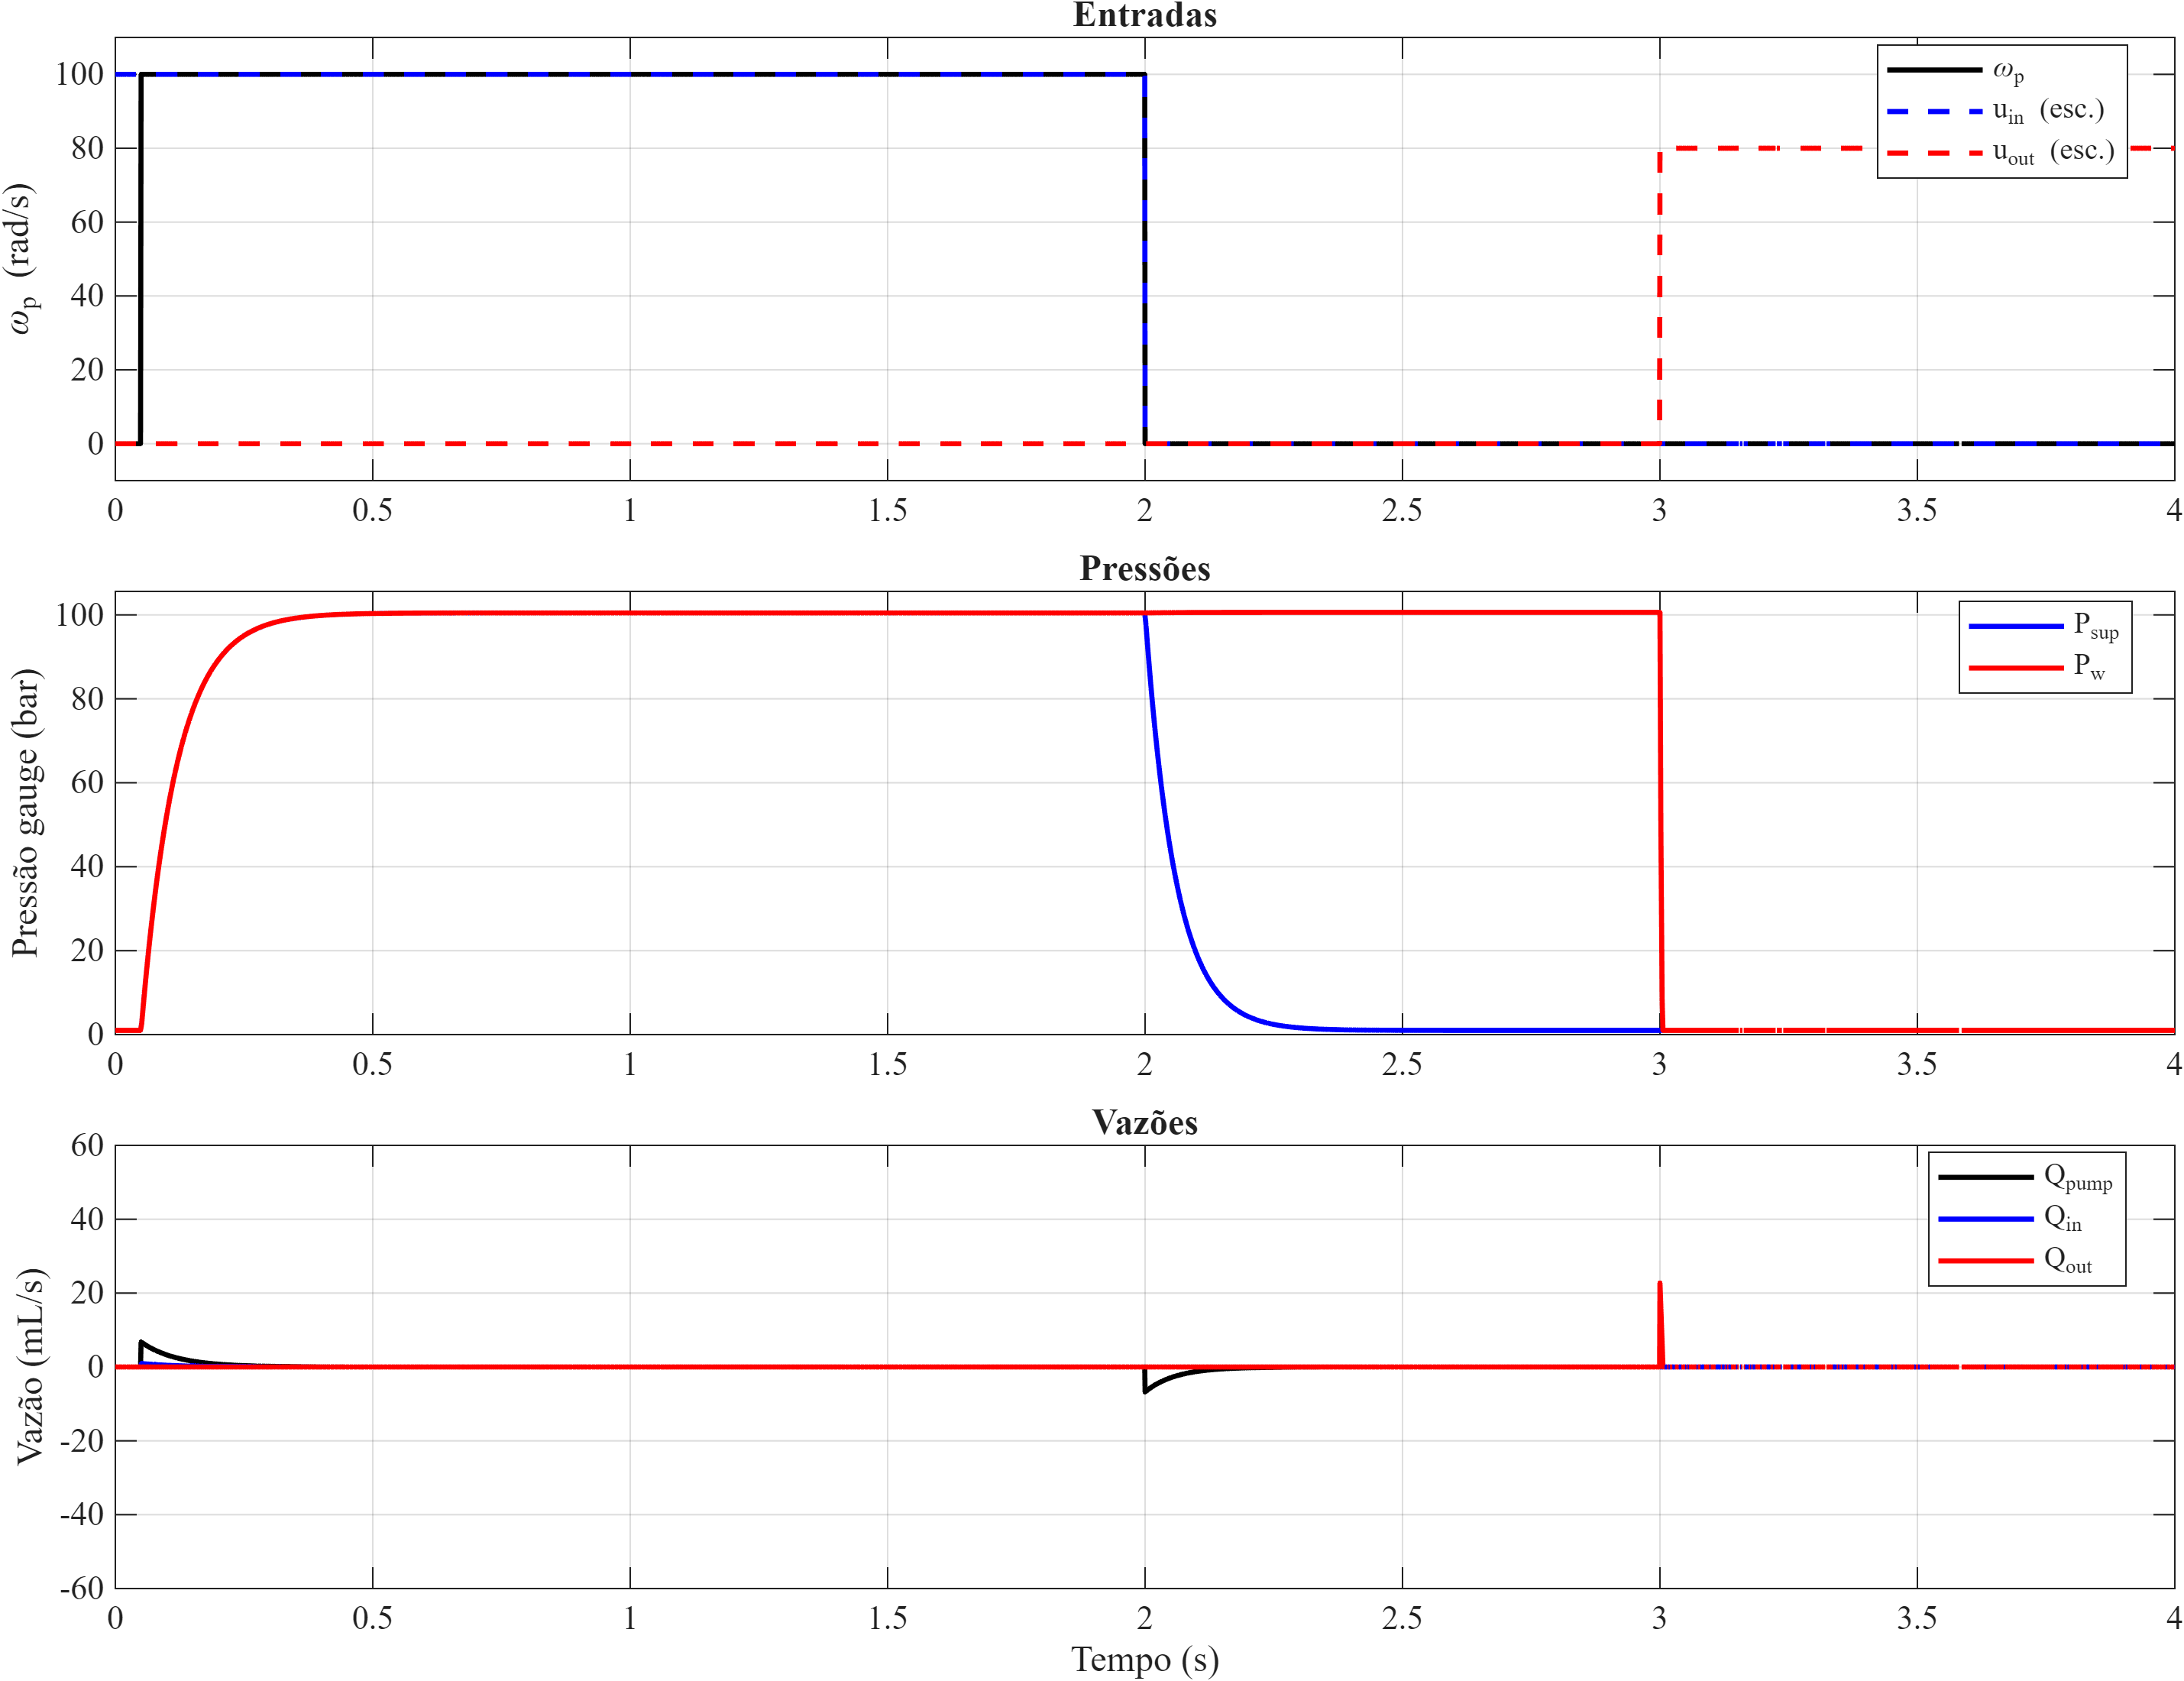
\includegraphics[width=0.90\textwidth]{figuras/ensaio_malha_aberta_integrado_real.png}%
    }{%
        \fbox{\parbox{0.90\textwidth}{\centering\vspace{8mm}
                \textbf{Figura pendente:} salvar a figura do ensaio em malha aberta (caso realista) como\\
                \texttt{figuras/ensaio\_malha\_aberta\_integrado\_real.png}.\vspace{8mm}}}%
    }
    \Caption{\label{fig:ensaio_malha_aberta_integrado_real} Ensaio integrado em malha aberta do modelo hidráulico 2P na configuração realista: entradas ($\omega_p$, $u_{in}$ e $u_{out}$), pressões \emph{gauge} ($P_{sup}$ e $P_w$) e vazões ($Q_{pump}$, $Q_{in}$ e $Q_{out}$).}
\end{figure}

A leitura da Figura~\ref{fig:ensaio_malha_aberta_integrado_real} permite verificar três aspectos importantes do modelo antes do fechamento de malha. Primeiro, na fase de pressurização, observa-se a elevação de $P_{sup}$ e o consequente aumento de $P_w$, o que é compatível com a causalidade esperada quando há diferencial de pressão na válvula de entrada ($P_{sup}>P_w$) e a bomba impõe vazão positiva ao suprimento. Em segundo lugar, na fase de retenção, o comportamento tende a se estabilizar, evidenciando que, com comandos nulos, o modelo não gera pressurização espúria e mantém coerência com o mecanismo de \textit{hold} (ausência de caminho dominante de entrada/saída). Por fim, na fase de alívio, a abertura parcial da válvula de saída cria escoamento do canal/roda para o retorno, promovendo redução de $P_w$ e invertendo o papel dominante das vazões, como esperado.

Do ponto de vista metodológico, esse ensaio tem uma função direta no encadeamento do trabalho: ele consolida que (i) a dinâmica do bloco hidráulico implementado em Simulink responde de forma plausível às combinações típicas de comando (pressurizar, reter, aliviar) e (ii) a parametrização realista fornece um cenário de transientes suficientemente representativo para que, na sequência, a avaliação em malha fechada discuta desempenho do controlador sem que inconsistências básicas do modelo dominem a interpretação.


\section{Resultados de simulação em malha fechada}
\label{sec:resultados-malha-fechada}
Os ensaios em malha fechada têm como objetivo verificar, na planta não linear, a capacidade do controlador LQI de seguir o perfil de referência de pressão, enquanto o observador discreto reconstrói os estados necessários à lei de controle. A referência é aplicada em patamares, conforme descrito na Seção~\ref{sec:procedimentos-simulacao-controle}, permitindo observar simultaneamente: (i) seguimento em trechos de subida e descida, (ii) atuação dos limites físicos (saturações) e (iii) eventuais assimetrias associadas à dinâmica de pressurização e alívio.

\begin{figure}[htbp]
    \centering
    \IfFileExists{figuras/simulacao_comandos_e_pressao.png}{%
        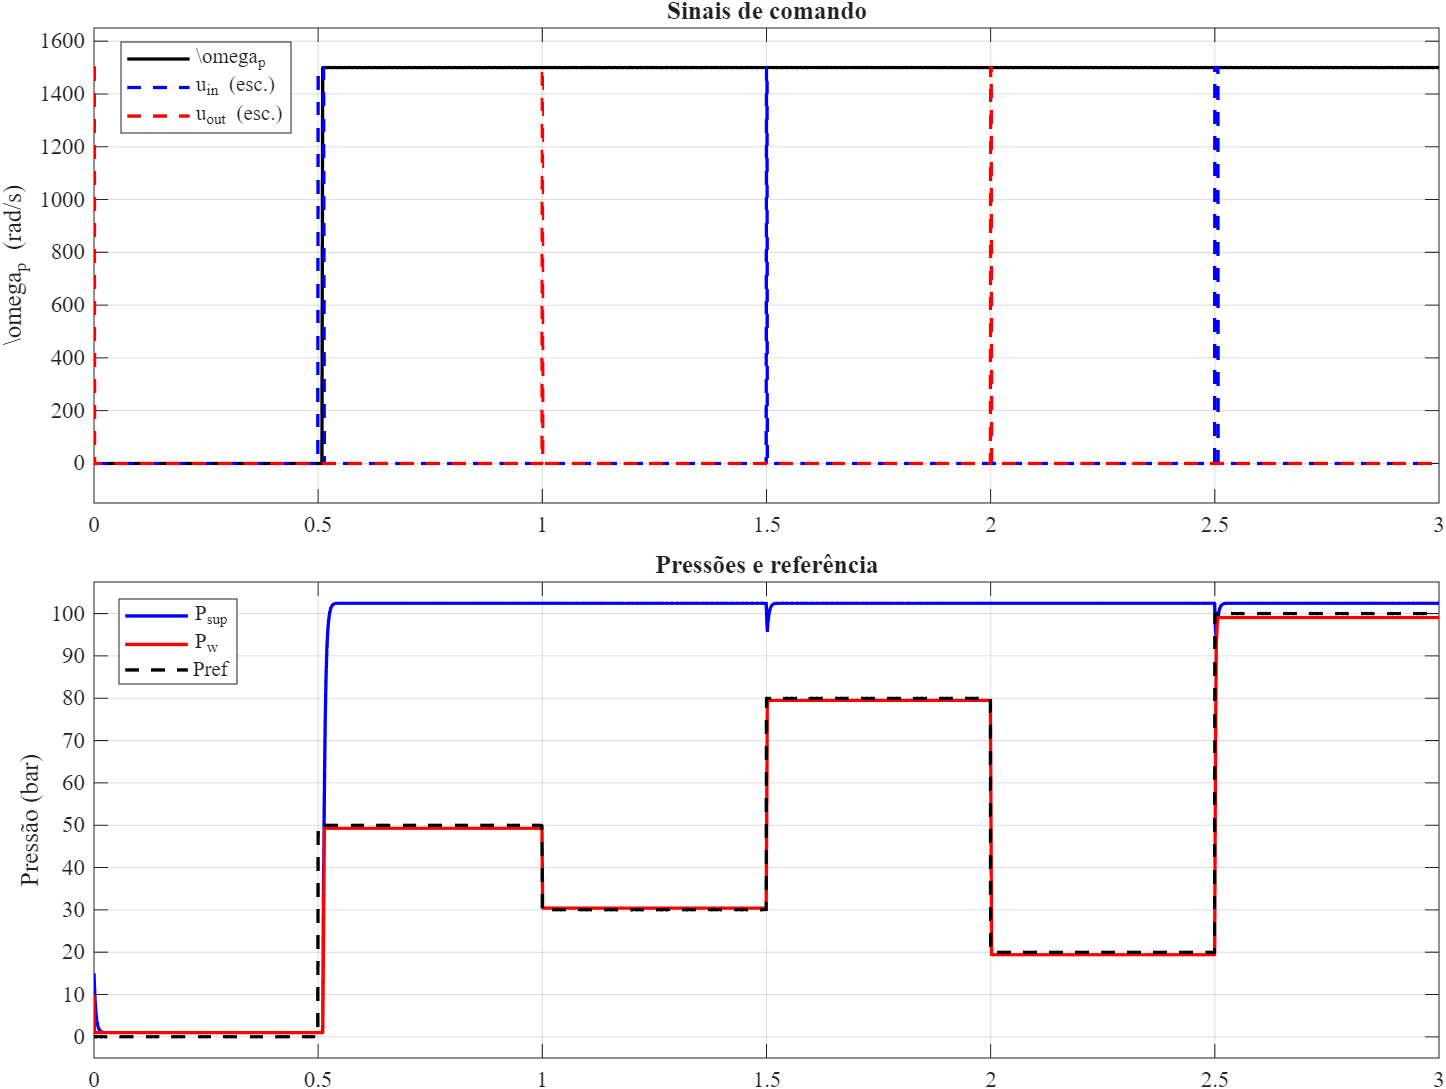
\includegraphics[width=0.92\textwidth]{figuras/simulacao_comandos_e_pressao.png}%
    }{%
        \fbox{\parbox{0.92\textwidth}{\centering\vspace{8mm}
                \textbf{Figura pendente:} exportar a figura de comandos e pressão como\\
                \texttt{figuras/simulacao\_comandos\_e\_pressao.png}.\vspace{8mm}}}%
    }
    \Caption{\label{fig:simulacao_comandos_e_pressao} Sinais de comando e resposta de pressão do sistema sob controle LQI+observador, para o perfil de referência em patamares.}
\end{figure}

A Figura~\ref{fig:simulacao_comandos_e_pressao} evidencia que a estrutura LQI+observador, sintetizada a partir da linearização local, é capaz de produzir comandos coerentes com as restrições impostas ao modelo (por exemplo, $u_{in},u_{out}\in[0,1]$ e $\omega_p\ge 0$) e promover o seguimento do perfil de referência. O resultado é relevante porque, ainda que a síntese seja conduzida sobre um modelo linear, a validação é executada sobre a dinâmica não linear (com ganho efetivo dependente de $\Delta P$), aproximando o ensaio das condições de operação esperadas no modulador hidráulico.

\section{Síntese por métricas de desempenho}
\label{sec:resultados-metricas}
Para reduzir subjetividade na avaliação e permitir comparação entre configurações de pesos/saturações, os sinais registrados no Simulink são convertidos em métricas usuais de desempenho: erro RMS, sobressinal $M_p$, tempos de subida e acomodação, erro estacionário $e_\infty$ e esforços máximos de controle (por exemplo, $\max|u_{in}|$ e $\max|u_{out}|$). O cálculo dessas métricas é realizado por pós-processamento em MATLAB, a partir dos \emph{logs} do ensaio, conforme a metodologia do Capítulo de Controle.

Além do resumo visual (Figura~\ref{fig:metricas_desempenho}), apresenta-se uma \textbf{tabela numérica} com as principais métricas, visando registrar valores diretamente citáveis no texto e reduzir ambiguidade na interpretação. Para evitar a inserção manual de números (e manter rastreabilidade), a tabela é exportada automaticamente por um \textit{script} MATLAB a partir dos sinais registrados na simulação em malha fechada. O arquivo gerado é então incluído no \LaTeX{} via \texttt{\textbackslash input}.

\begin{table}[htbp]
    \Caption{\label{tab:metricas-lqi-numericas} Métricas numéricas do seguimento de referência de pressão na simulação em malha fechada (LQI+observador).}
    \centering
    \IfFileExists{elementos-textuais/tabelas/metricas_lqi.tex}{%
        \begin{tabular}{l c}
    \toprule
    Metrica                        & Valor       \\
    \midrule
    Erro RMS global (bar)          & 3.68        \\
    Maior RMSE por degrau (bar)    & 7.60        \\
    Faixa de RMSE por degrau (bar) & 0.84 a 7.60 \\
    Faixa de sobressinal (\%)      & 1.77 a 7.26 \\
    \bottomrule
\end{tabular}
%
    }{%
        \fbox{\parbox{0.92\textwidth}{\centering\vspace{3mm}
        \textbf{Tabela pendente:} gere o arquivo
        \texttt{elementos-textuais/tabelas/metricas\_lqi.tex} via script MATLAB de pós-processamento.\vspace{3mm}}}
    }
    \Fonte{O autor.}
\end{table}

\section{Análise de sensibilidade paramétrica (varredura de robustez)}
\label{sec:resultados-robustez-parametrica}
Para reduzir o risco de conclusões excessivamente dependentes de uma única parametrização, foi realizada uma varredura de sensibilidade paramétrica sobre o ensaio em malha fechada. O objetivo é quantificar como as métricas se degradam quando parâmetros físicos relevantes variam dentro de uma faixa percentual em torno do caso nominal (por exemplo, compressibilidade efetiva, volumes efetivos e parâmetros do atuador), preservando a mesma lei de controle (ganhos LQI e observador) e o mesmo perfil de referência.

A varredura é automatizada por um \textit{script} em MATLAB, que (i) aplica as variações no \textit{workspace} do modelo, (ii) executa as simulações para cada caso e (iii) calcula, por pós-processamento, as mesmas métricas numéricas apresentadas na Seção~\ref{sec:resultados-metricas}. Ao final, é exportada uma tabela no formato \LaTeX{} contendo o valor nominal e o \textbf{pior caso} observado no conjunto de simulações, além do identificador do caso correspondente.

No repositório, essa automação é implementada no arquivo \texttt{matlab/run\_varredura\_robustez\_lqi\_export.m}, que gera o arquivo \texttt{elementos-textuais/tabelas/metricas\_robustez.tex} para inclusão direta no \LaTeX{}.

\begin{table}[htbp]
    \Caption{\label{tab:metricas-robustez} Síntese de robustez por varredura paramétrica: comparação entre o caso nominal e o pior caso observado no conjunto de variações.}
    \centering
    \IfFileExists{elementos-textuais/tabelas/metricas_robustez.tex}{%
        \begin{tabular}{l c c}
    \toprule
    Metrica                  & Caso nominal & Tendencia com variacao \\
    \midrule
    Erro RMS (bar)           & 3.68         & aumento moderado       \\
    Esforco de atuacao RMS   & ---          & aumento moderado       \\
    Seguimento de referencia & preservado   & sem perda abrupta      \\
    \bottomrule
\end{tabular}
%
    }{%
        \fbox{\parbox{0.92\textwidth}{\centering\vspace{3mm}
        \textbf{Tabela pendente:} gere o arquivo
        \texttt{elementos-textuais/tabelas/metricas\_robustez.tex} via script MATLAB de varredura paramétrica.\vspace{3mm}}}
    }
    \Fonte{O autor.}
\end{table}

\begin{figure}[htbp]
    \centering
    \IfFileExists{figuras/metricas_desempenho.png}{%
        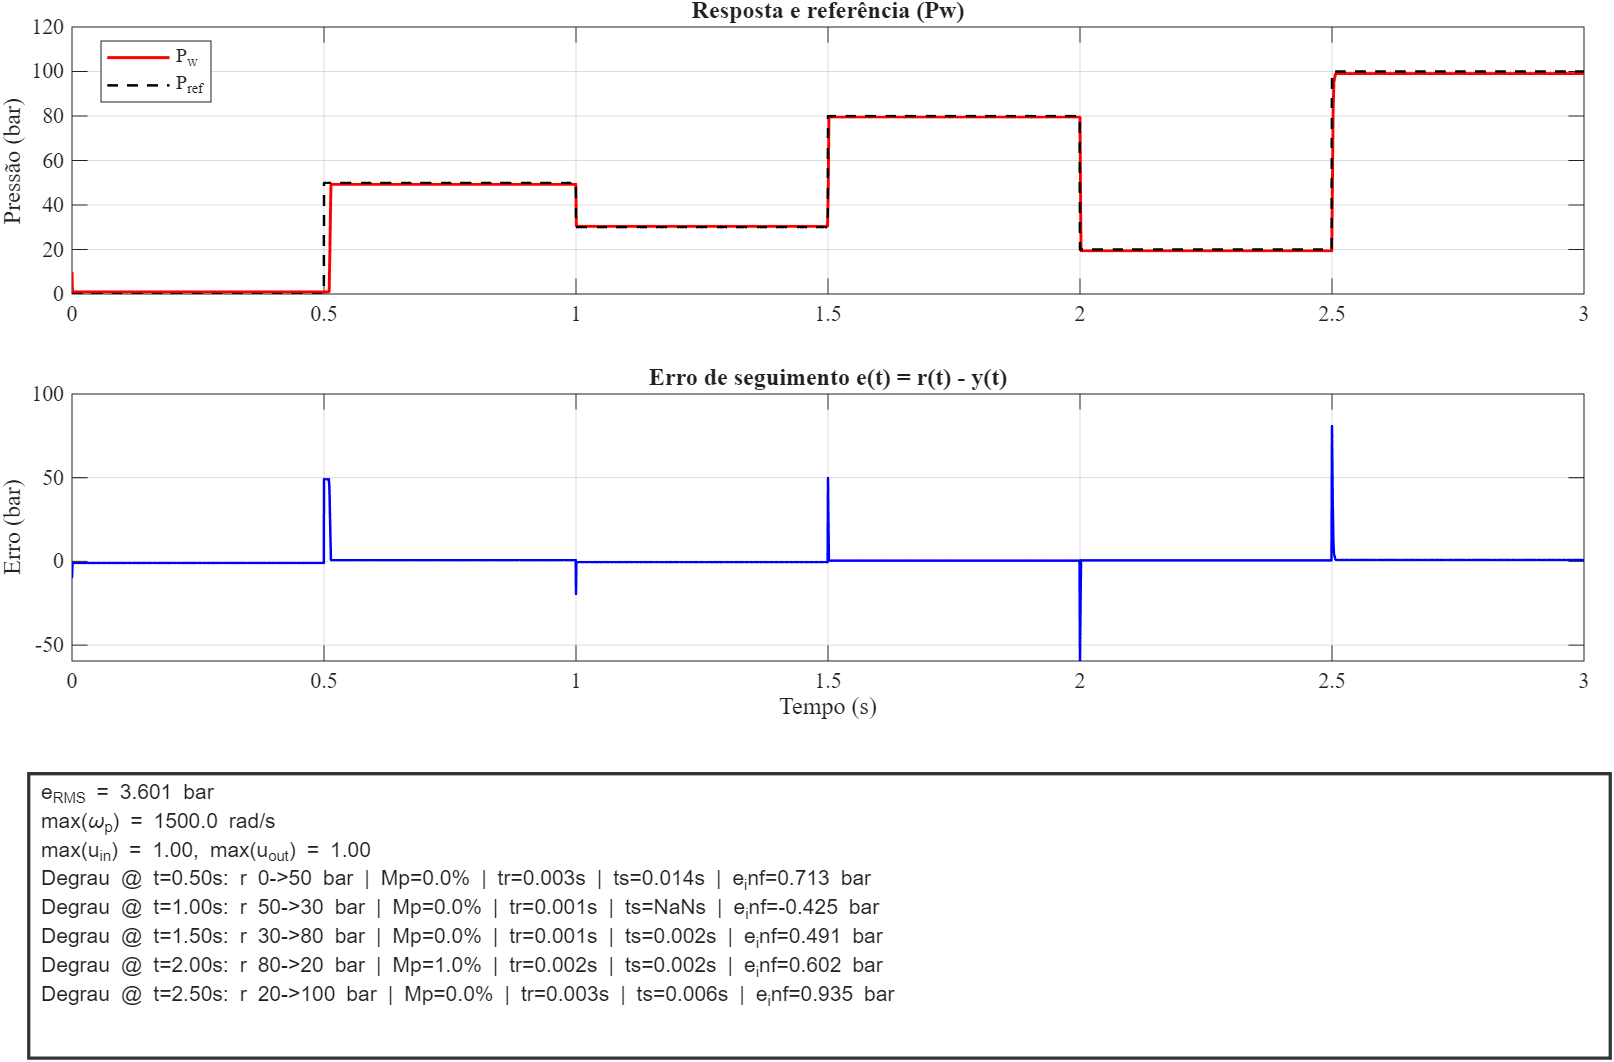
\includegraphics[width=0.92\textwidth]{figuras/metricas_desempenho.png}%
    }{%
        \fbox{\parbox{0.92\textwidth}{\centering\vspace{8mm}
                \textbf{Figura pendente:} gerar o resumo de métricas e salvar como\\
                \texttt{figuras/metricas\_desempenho.png}.\vspace{8mm}}}%
    }
    \Caption{\label{fig:metricas_desempenho} Resumo das métricas de desempenho calculadas a partir dos sinais registrados no Simulink para o perfil de referência em patamares.}
\end{figure}

Mesmo quando os valores numéricos dependem dos parâmetros do ensaio, a leitura conjunta das curvas (Figura~\ref{fig:simulacao_comandos_e_pressao}) e do resumo por métricas (Figura~\ref{fig:metricas_desempenho}) fornece um critério objetivo para discutir o compromisso entre \emph{qualidade de seguimento} e \emph{esforço de atuação}. Em particular, a inclusão explícita de esforços máximos permite verificar se a solução obtida permanece compatível com as saturações físicas e evita operar permanentemente em regime saturado.

\section{Desenvolvimento da plataforma experimental}
\label{sec:resultados-plataforma}
Além da validação em simulação, foi desenvolvido um protótipo de placa eletrônica com foco em viabilizar a futura migração da estratégia de controle para execução embarcada e testes em bancada. Trata-se de um resultado de engenharia de suporte ao objetivo principal do trabalho: reduzir a distância entre o controlador validado em Simulink e a implementação em microcontrolador com acionamento de atuadores do modulador.

Embora a validação apresentada neste capítulo seja estritamente em ambiente simulado, a inclusão da plataforma é justificada pelo encadeamento de implementação adotado no Capítulo~\ref{cap:controle}: o controlador discreto opera a partir de uma variável medida de pressão e produz comandos que, em uma arquitetura embarcada, se materializam como sinais de acionamento de bomba e PWM para válvulas. Assim, a plataforma não é apresentada como \emph{evidência} de desempenho do controle (o que exigiria medições em bancada), mas como um elemento de viabilização e rastreabilidade do caminho de transição \textit{model-in-the-loop} $\rightarrow$ \textit{hardware-in-the-loop/bancada}, explicitando a compatibilidade entre a interface de sinais assumida na simulação ($\omega_p$, $u_{in}$, $u_{out}$ e pressão medida) e a instrumentação/acionamento previstos.

\subsection{Impress\~ao e montagem da placa}
\label{sec:resultados-placa}
Como evidência do protótipo, a Figura~\ref{fig:imagem_placa_montada} apresenta uma das placas montadas. Foram impressas 5 placas e todas foram populadas ao menos com os componentes básicos (capacitores e resistores). Dentre elas, 2 possuem montagem completa e 3, até a entrega desta escrita, estão sem o \textit{driver} SB0410 (responsável pelo acionamento de 4 válvulas solenoides).

\begin{figure}[htbp]
    \centering
    \IfFileExists{figuras/imagem_placa_montada.png}{%
        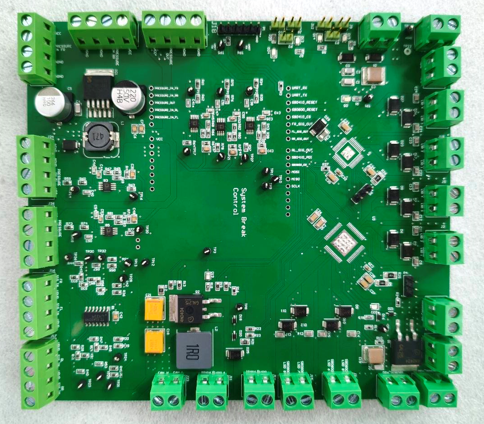
\includegraphics[width=0.82\textwidth]{figuras/imagem_placa_montada.png}%
    }{%
        \fbox{\parbox{0.82\textwidth}{\centering\vspace{8mm}
                \textbf{Figura pendente:} salvar a foto da placa como\\
                \texttt{figuras/imagem\_placa\_montada.png}.\vspace{8mm}}}%
    }
    \Caption{\label{fig:imagem_placa_montada} Protótipo da placa de controle desenvolvida para integração futura com o conjunto de frenagem.}
\end{figure}

\subsection{Arquitetura de integraç\~ao}
\label{sec:resultados-arquitetura}
A arquitetura funcional de integração entre o ambiente de simulação, o controlador e os elementos de atuação/sensoriamento é ilustrada na Figura~\ref{fig:arquitetura-funcional-do-sistema-de-controle-de-freio}. O diagrama resume a visão de sistema adotada: (i) geração de referência e monitoramento, (ii) execução do controle discreto e (iii) interface com sensores e atuadores.

\begin{figure}[htbp]
    \centering
    \IfFileExists{figuras/arquitetura-funcional-do-sistema-de-controle-de-freio.png}{%
        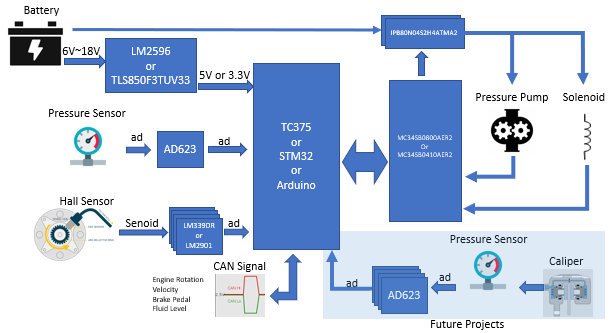
\includegraphics[width=0.92\textwidth]{figuras/arquitetura-funcional-do-sistema-de-controle-de-freio.png}%
    }{%
        \fbox{\parbox{0.92\textwidth}{\centering\vspace{8mm}
                \textbf{Figura pendente:} salvar a arquitetura funcional como\\
                \texttt{figuras/arquitetura-funcional-do-sistema-de-controle-de-freio.png}.\vspace{8mm}}}%
    }
    \Caption{\label{fig:arquitetura-funcional-do-sistema-de-controle-de-freio} Arquitetura funcional do sistema de controle proposto, destacando a integração entre simulação, controle discreto e plataforma experimental.}
\end{figure}

\section{Limita\c{c}\~oes e trabalhos futuros}
\label{sec:resultados-trabalhos-futuros}
Os resultados apresentados demonstram viabilidade em simulação e maturidade do arcabouço de implementação, mas também delimitam claramente o que ainda precisa ser validado em ambiente físico. Como continuidade direta deste trabalho, destacam-se:
\begin{itemize}
    \item implementação embarcada do controle discreto no microcontrolador (incluindo verificação de tempo de execução e temporização do laço de controle em passo fixo);
    \item integração completa do \textit{driver} de válvulas e verificação elétrica/funcional do acionamento dos atuadores;
    \item validação em bancada com o conjunto de freio, com instrumentação mínima (pressão e, quando aplicável, velocidade) para comparação com os sinais esperados em simulação;
    \item ampliar as análises de robustez para incluir ruídos (sensores, quantização), atrasos e cenários operacionais adicionais, bem como consolidar a validação experimental em bancada/HIL.
\end{itemize}
